


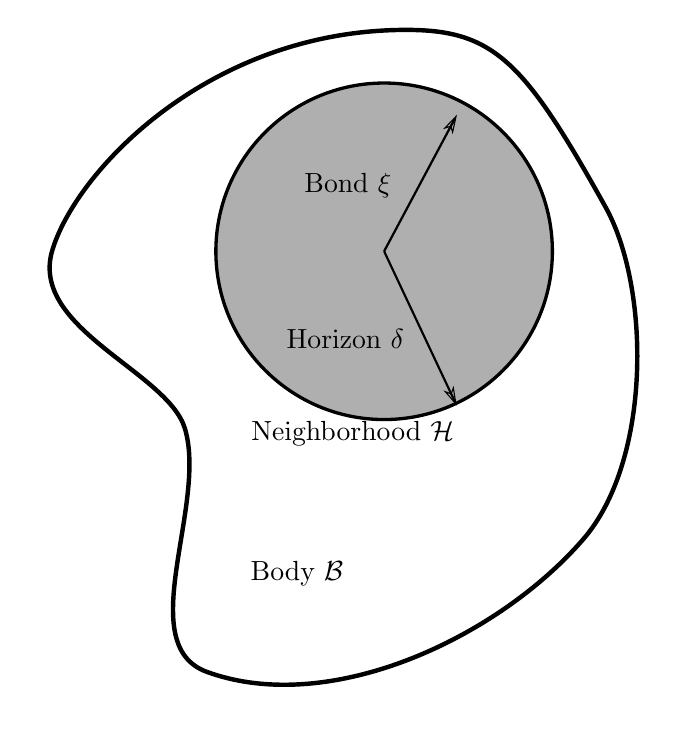
\begin{tikzpicture}[y=0.80pt, x=0.8pt,yscale=-1, inner sep=0pt, outer sep=0pt]
\begin{scope}[shift={(0,-552.36223)}]
  \path[shift={(0,552.36223)},draw=black,fill=black,line join=round,miter
    limit=4.00,fill opacity=0.314,line width=1.200pt] (336.0000,180.0000) ..
    controls (336.0000,221.9736) and (301.9736,256.0000) .. (260.0000,256.0000) ..
    controls (218.0264,256.0000) and (184.0000,221.9736) .. (184.0000,180.0000) ..
    controls (184.0000,138.0264) and (218.0264,104.0000) .. (260.0000,104.0000) ..
    controls (301.9736,104.0000) and (336.0000,138.0264) .. (336.0000,180.0000) --
    cycle;
  \path[shift={(0,552.36223)},draw=black,line join=miter,line cap=butt,miter
    limit=4.00,line width=1.600pt] (270.0000,80.0000) .. controls
    (309.5854,80.0000) and (323.3333,94.1417) .. (360.0000,160.0000) .. controls
    (380.3169,196.4920) and (380.8463,274.3527) .. (350.0000,310.0000) .. controls
    (311.3497,354.6659) and (235.5187,390.1635) .. (180.0000,370.0000) .. controls
    (146.1103,357.6918) and (180.4483,294.5084) .. (170.0000,260.0000) .. controls
    (162.2724,234.4776) and (100.0000,215.0000) .. (110.0000,180.0000) .. controls
    (120.0000,145.0000) and (180.0000,80.0000) .. (270.0000,80.0000) -- cycle;
    \path[color=black,fill=black,line width=0.800pt] (260.4375,732.1435) --
      (259.5625,732.5810) -- (291.5625,800.5810) -- (292.4375,800.1435) --
      (260.4375,732.1435) -- cycle;
    \path[draw=black,even odd rule,line width=0.400pt] (290.2968,796.7430) --
      (287.6356,795.7849) -- (292.4258,801.2671) -- (291.2549,794.0817) --
      (290.2968,796.7430) -- cycle;
  \path[fill=black] (216,776.36224) node[above right] (text7637) {Horizon
    $\delta$};
  \path[fill=black] (200,820.36224) node[above right] (text7641) {Neighborhood
    $\mathcal{H}$};
  \path[shift={(0,552.36223)},fill=black] (199.75768,331.30453) node[above right]
    (text7645) {Body $\mathcal{B}$};
    \path[color=black,fill=black,line width=0.800pt] (291.5625,672.1122) --
      (259.5625,732.1122) -- (260.4375,732.6122) -- (292.4375,672.6122) --
      (291.5625,672.1122) -- cycle;
    \path[draw=black,even odd rule,line width=0.400pt] (290.1177,675.8916) --
      (290.9412,678.5975) -- (292.4706,671.4799) -- (287.4118,676.7152) --
      (290.1177,675.8916) -- cycle;
  \path[fill=black] (224,708.36224) node[above right] (text3416) {Bond
    $\boldsymbol{\xi}$};
\end{scope}

\end{tikzpicture}

